\section{Study of using pose with higher frequency}

In this study, we are investigating the effect that pose estimation 
uncertainty brings to tracking performance. 
In SLAM pose-based control, the pose estimation errors immediately cause worse tracking performance. 
The design of trajectory servoing intends to improve the performance 
by less frequently requesting robot poses and shifting to the image domain. 
We already have the comparison of SLAM and TS in the paper. 
To further show the effect of pose estimation uncertainty, 
we conduct ablation studies about tracking performance 
when trajectory servoing more frequently using SLAM poses.

\subsection{Feature replenishment threshold $\tau_{fr}$ \label{sec:thresh}}

From \S III.A in the paper, the feature replenishment threshold $\tau_{fr}$ 
controls the frequency of feature trajectory regeneration and 
robot pose requesting with long distance trajectories.
In the simulation, we conduct an ablation study about the influence of 
varying $\tau_{fr}$. 
The same two trajectory tracking performance metrics are used: 
average lateral error (ALE) and terminal error (TE).
The number of feature trajectory regeneration per length is also recorded.
Outcomes of averages over all trajectory templates are included in 
Table \ref{tab:regThresh} and Fig. \ref{fig:regThresh}

With smaller $\tau_{fr}$, trajectory servoing uses less number of tracked features, 
and works similar to pure IBVS. 
The computed control could be unstable and have oscillations, which reduces 
the tracking performance. 
In contrast, if $\tau_{fr}$ is significantly large, trajectory servoing 
will more frequently trigger feature replenishment. 
The performance will be more related to pose estimation accuracy, 
and be close to SLAM pose-based control.
More pose estimation errors cause worse performance.

\begin{figure*}[h]
\begin{minipage}[t]{\textwidth}
\centering
%\vspace*{-1.45in}
\captionof{table}{ Raw data from ablation study of feature replenishment $\tau_{fr}$ \label{tab:regThresh}}
\vspace*{-0.5em}
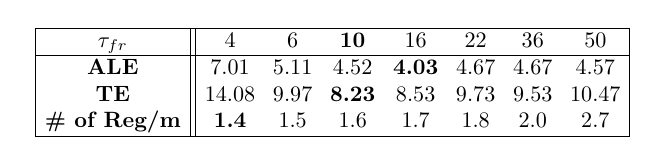
\begin{tikzpicture}[inner sep=0pt,outer sep=0pt,scale=1, every node/.style={scale=0.8}]
    % 
  \node[anchor=north west] (sim_thresh) at (0, 0pt)
  {
  \setlength{\tabcolsep}{4pt}
  \begin{tabular}{|c||ccccccc|}
  \hline 
  \textbf{$\tau_{fr}$} & 4 & 6 & \textbf{10} & 16 & 22 & 36 & 50 \\ 
  \hline 
  \textbf{ALE}  & 7.01 & 5.11 & 4.52 & \textbf{4.03} & 4.67 & 4.67 & 4.57 \\ 
  \textbf{TE}   & 14.08 & 9.97 & \textbf{8.23} & 8.53 & 9.73 & 9.53 & 10.47  \\ 
  \textbf{\# of Reg/m} & \textbf{1.4} & 1.5 & 1.6 & 1.7 & 1.8 & 2.0 & 2.7 \\ 
  \hline 
  \end{tabular}
  };       

\end{tikzpicture}
\end{minipage}
\vspace*{-0.5em}
\end{figure*}

\begin{figure*}[h]
\begin{minipage}[t]{0.49\textwidth}
\centering
\begin{tikzpicture}[inner sep=0pt,outer sep=0pt]
	  \node[anchor=south west] (pop) at (0in, 0in)
      {{\includegraphics[height=2.2in,clip=true,trim=0in 0in
      0in 0in]{figs/tau_num_reg.png}}};
\end{tikzpicture}
\end{minipage}
\hfill
\begin{minipage}[t]{0.49\textwidth}
\centering
\begin{tikzpicture}[inner sep=0pt,outer sep=0pt]
	  \node[anchor=south west] (pop) at (0in, 0in)
      {{\includegraphics[height=2.2in,clip=true,trim=0in 0in
      0in 0in]{figs/tau_ale_te.png}}};
\end{tikzpicture}
\end{minipage}
\vspace*{-0.5em}
\caption{Ablation study plots of feature replenishment $\tau_{fr}$ \label{fig:regThresh}}
\vspace*{-0.5em}
\end{figure*}

\subsection{Incremental Trajectory Servoing}

In order to further investigate the effect that pose estimation uncertainty 
brings to tracking performance. 
The trajectory servoing system is modified to use robot pose information 
in every control loop and recomputes the desired feature set 
for the next pose on the given trajectory. 
The feature trajectory will not be precomputed at the beginning.
This version is called {\em Incremental Trajectory Servoing} (I-TS).
Unlike the regular feature replenishment in \S III.A that is triggered 
by $\tau_{fr}$, desired feature regeneration is triggered by time.
By doing this modification, trajectory servoing works similar to 
SLAM pose-based control, but shifting feedback to the image domain. 

We applied the same simulation benchmark and metrics (i.e. ALE and TE) 
to compare tracking performance. 
The benchmark is only tested with long distance trajectories, 
because SLAM pose estimation uncertainty is not explicit with short distance 
trajectories. Tables \ref{tab:longITS}(a,b) gives outcomes for the two metrics.
I-TS has worse ALE and TE than TS and is similar to SLAM.
It shows that frequently using SLAM pose information will introduce more 
uncertainty that potentially do harm to the tracking.

\begin{figure*}[h]
\begin{minipage}[t]{\textwidth}
\centering
%\vspace*{-1.45in}
\captionof{table}{ Incremental Trajectory Servoing Outcomes.\label{tab:longITS}}
\vspace*{-0.5em}
\begin{tikzpicture}[inner sep=0pt,outer sep=0pt,scale=1, every node/.style={scale=0.8}]
    % sim ALE
	\node[anchor=north west] (sim_ale) at (0, 0pt)
    {
    \setlength{\tabcolsep}{4pt}
    \begin{tabular}{|c||c|ccc|}
    \hline 
    \textbf{Seq.} & PO & SLAM & TS & I-TS \\ 
    \hline 
%       &       &       & SLAM  & $\neg$SLAM \\
    LRU & 0.53  & 3.88  & 4.00  & 3.56 \\ 
    LLU & 0.86  & 8.21  & 5.18  & 7.68 \\ 
    LST & 1.13  & 5.03  & 3.00  & 4.19 \\ 
    LZZ & 1.06  & 7.54  & 5.90  & 9.72 \\ 
    \hline 
    \textbf{Avg.} & 0.90 & 6.17 & \textbf{4.52} & 6.29 \\
    %\textbf{Std. ATE} & 0.0000 & 0.0000 & 0.0000 \\
%    & \textcolor{white}{$v,\omega$} & & & \\
    \hline 
    \end{tabular}
    };
    
    \node[anchor=south, text width=5cm, text centered] (sim_ale_cap) 
    at ($(sim_ale.north) + (0pt, 2pt)$)
    {\normalsize \textbf{(a)} Sim {ALE} (cm)};
      
    % sim TE
    \node[anchor=west] (sim_te) at ($(sim_ale.east) + (5pt, 0)$)
    {
    \setlength{\tabcolsep}{4pt}
    \begin{tabular}{|c||c|ccc|}
    \hline 
    \textbf{Seq.} & PO & SLAM & TS & I-TS \\ 
    \hline 
%       &       &       & SLAM  & $\neg$SLAM \\
    LRU & 8.57  & 10.66   & 6.42  & 8.82 \\ 
    LLU & 5.54  & 29.48  & 15.75 & 24.3 \\ 
    LST & 6.01  & 7.60  & 1.76  & 10.45 \\ 
    LZZ & 7.83  & 9.28   & 9.00  & 9.91 \\ 
    \hline 
    \textbf{Avg.} & 6.99 & 14.26 & \textbf{8.23} & 13.37 \\ 
    %\textbf{Std. ATE} & 0.0000 & 0.0000 & 0.0000 \\
%    & \textcolor{white}{$v,\omega$} & & & \\
    \hline 
    \end{tabular}
    };
    
	\node[anchor=south, text width=5cm, text centered] (sim_ale_p_cap) 
    at ($(sim_te.north) + (0pt, 2pt)$)
    {\normalsize \textbf{(b)} Sim {TE} (cm)};        

\end{tikzpicture}
\end{minipage}
\vspace*{-1.5em}
\end{figure*}

\subsection{Conclusion}

The above two studies shows the effect of pose estimation uncertainty 
when using SLAM poses with higher frequency.
In addition, the results of TS+PO in the paper also 
indicate the improved performance with more accurate pose information. 
Overall, pose estimation uncertainty can lead to worse trajectory tracking performance. 
Our trajectory servoing design can reduce the effect of this uncertainty 
and have better tracking results.
